%%%%%%%%%%%%%%%%%%%%%%%%%%%%%%%%%%%%%%%%%%%%%%%%%%%%%%%%%%%%%%%%%%%%%%%%%%%%%%%%%%
\begin{frame}[fragile]\frametitle{}
\begin{center}
{\Large Decision Tree  - Synthetic Dataset}

{\tiny (Ref: mlcourse.ai Demo 3 – Open Machine Learning Course) }

\end{center}

\end{frame}

%%%%%%%%%%%%%%%%%%%%%%%%%%%%%%%%%%%%%%%%%%%%%%%%%%%%%%%%%%
\begin{frame}[fragile]\frametitle{Import Libraries}	
\begin{lstlisting}
from matplotlib import pyplot as plt
plt.rcParams['figure.figsize'] = (10, 8)
import seaborn as sns
import numpy as np
import pandas as pd
from sklearn.preprocessing import LabelEncoder
import collections
from sklearn.model_selection import GridSearchCV
from sklearn import preprocessing
from sklearn.tree import DecisionTreeClassifier, export_graphviz
from sklearn.ensemble import RandomForestClassifier
from sklearn.metrics import accuracy_score
from ipywidgets import Image
from io import StringIO
import pydotplus #pip install pydotplus
\end{lstlisting}
\end{frame}

%%%%%%%%%%%%%%%%%%%%%%%%%%%%%%%%%%%%%%%%%%%%%%%%%%%%%%%%%%
\begin{frame}[fragile]\frametitle{Problem Info}	
\begin{itemize}
\item Binary classification
\item Person A is deciding whether they will go on a second date with Person B. 
\item It will depend on their looks, eloquence, alcohol consumption (only for example), and how much money was spent on the first date.
\end{itemize}
\end{frame}



%%%%%%%%%%%%%%%%%%%%%%%%%%%%%%%%%%%%%%%%%%%%%%%%%%%%%%%%%%
\begin{frame}[fragile]\frametitle{Creating the Artificial dataset}	
Features and Target ("Will\_go") are defined as:
\begin{lstlisting}
df_train = {}
features = ['Looks', 'Alcoholic_beverage','Eloquence','Money_spent']
df_train['Looks'] = ['handsome', 'handsome', 'handsome', 'repulsive',
                         'repulsive', 'repulsive', 'handsome'] 
df_train['Alcoholic_beverage'] = ['yes', 'yes', 'no', 'no', 'yes', 'yes', 'yes']
df_train['Eloquence'] = ['high', 'low', 'average', 'average', 'low',
                                   'high', 'average']
df_train['Money_spent'] = ['lots', 'little', 'lots', 'little', 'lots',
                                  'lots', 'lots']
df_train['Will_go'] = LabelEncoder().fit_transform(['+', '-', '+', '-', '-', '+', '+'])
\end{lstlisting}
\end{frame}

%%%%%%%%%%%%%%%%%%%%%%%%%%%%%%%%%%%%%%%%%%%%%%%%%%%%%%%%%%
\begin{frame}[fragile]\frametitle{Create Training Data-frame}	
\begin{lstlisting}
# Create dataframe with dummy variables
def create_df(dic, feature_list):
    out = pd.DataFrame(dic)
    out = pd.concat([out, pd.get_dummies(out[feature_list])], axis = 1)
    out.drop(feature_list, axis = 1, inplace = True)
    return out
	
df_train = create_df(df_train, features)
\end{lstlisting}
\end{frame}

%%%%%%%%%%%%%%%%%%%%%%%%%%%%%%%%%%%%%%%%%%%%%%%%%%%%%%%%%%%%%%%%%%%%%%%%%%%%%%%%%%
\begin{frame}[fragile]\frametitle{Create Data-frame}	
\begin{center}
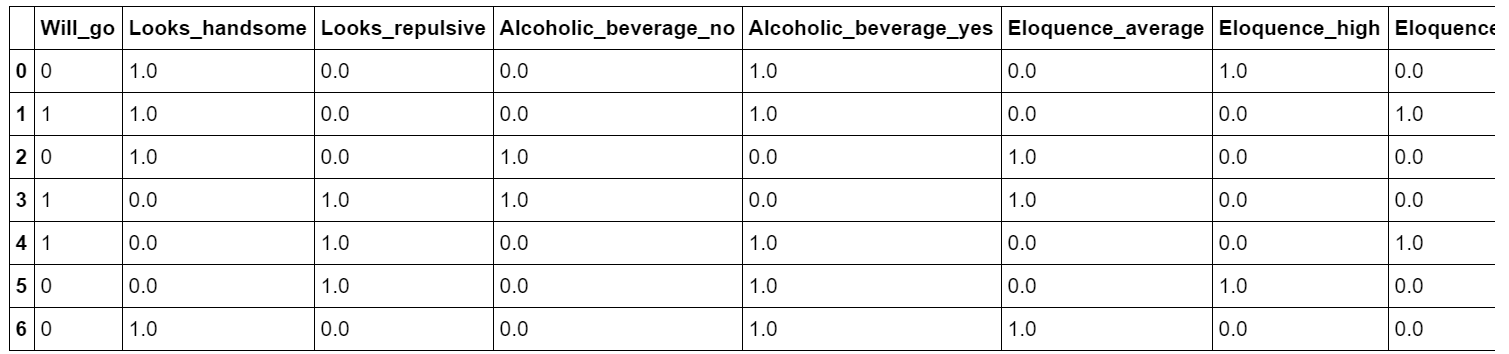
\includegraphics[width=\linewidth,keepaspectratio]{mlcourse9}
\end{center}
\end{frame}

%%%%%%%%%%%%%%%%%%%%%%%%%%%%%%%%%%%%%%%%%%%%%%%%%%%%%%%%%%
\begin{frame}[fragile]\frametitle{Create Testing Data-frame}	
\begin{lstlisting}
df_test = {}
df_test['Looks'] = ['handsome', 'handsome', 'repulsive'] 
df_test['Alcoholic_beverage'] = ['no', 'yes', 'yes']
df_test['Eloquence'] = ['average', 'high', 'average']
df_test['Money_spent'] = ['lots', 'little', 'lots']
df_test = create_df(df_test, features)
\end{lstlisting}

\begin{center}
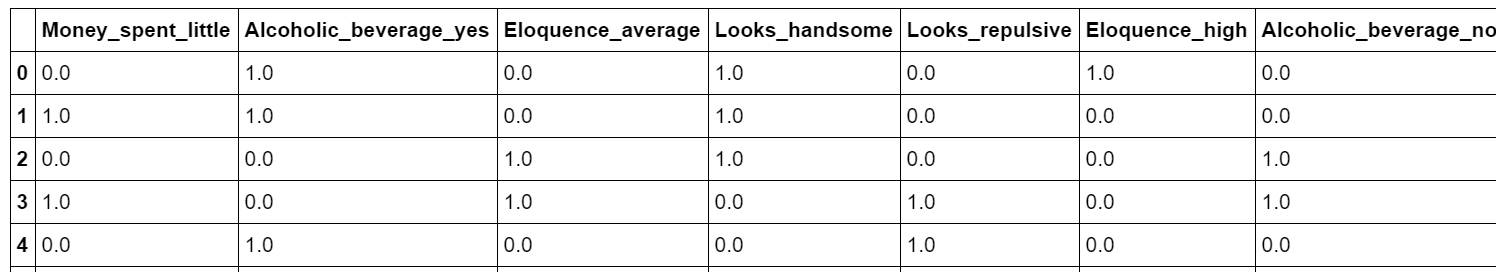
\includegraphics[width=\linewidth,keepaspectratio]{mlcourse10}
\end{center}
\end{frame}


%%%%%%%%%%%%%%%%%%%%%%%%%%%%%%%%%%%%%%%%%%%%%%%%%%%%%%%%%%
\begin{frame}[fragile]\frametitle{Create Datasets}	
\begin{lstlisting}
# Some feature values are present in train and absent in test and vice-versa.
y = df_train['Will_go']
def intersect_features(train, test):
    common_feat = list( set(train.keys()) & set(test.keys()))
    return train[common_feat], test[common_feat]

df_train, df_test = intersect_features(train=df_train, test=df_test)
\end{lstlisting}
\begin{center}
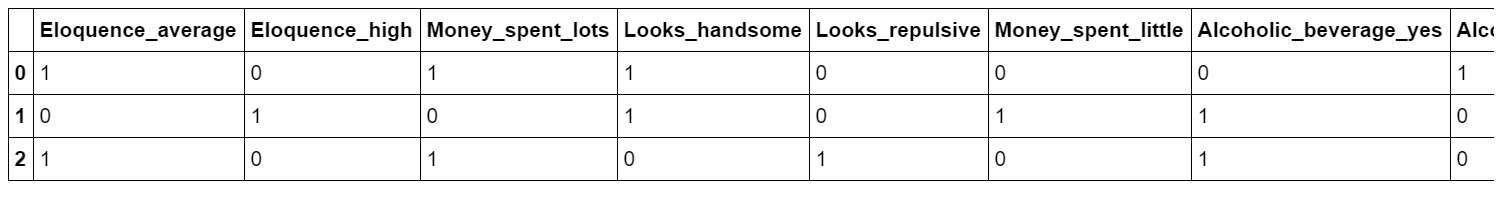
\includegraphics[width=\linewidth,keepaspectratio]{mlcourse11}
\end{center}
\end{frame}

%%%%%%%%%%%%%%%%%%%%%%%%%%%%%%%%%%%%%%%%%%%%%%%%%%%%%%%%%%
\begin{frame}[fragile]\frametitle{Question 1}	
What is the entropy  $S_0$  of the initial system? By system states, we mean values of the binary feature ``Will\_go'' - 0 or 1 - two states in total.
\end{frame}

%%%%%%%%%%%%%%%%%%%%%%%%%%%%%%%%%%%%%%%%%%%%%%%%%%%%%%%%%%
\begin{frame}[fragile]\frametitle{Solution 1}	
$S_0 = -\frac{3}{7}\log_2{\frac{3}{7}}-\frac{4}{7}\log_2{\frac{4}{7}} = 0.985$
\end{frame}

%%%%%%%%%%%%%%%%%%%%%%%%%%%%%%%%%%%%%%%%%%%%%%%%%%%%%%%%%%
\begin{frame}[fragile]\frametitle{Question 2}	
\begin{itemize}
\item Let's split the data by the feature ``Looks\_handsome''. 
\item  What is the entropy  $S_1$  of the left group - the one with ``Looks\_handsome''. 
 \item What is the entropy  $S_2$  in the opposite group? 
 \item What is the information gain (IG) if we consider such a split?
\end{itemize}
 
 \end{frame}

%%%%%%%%%%%%%%%%%%%%%%%%%%%%%%%%%%%%%%%%%%%%%%%%%%%%%%%%%%
\begin{frame}[fragile]\frametitle{Solution 2}	
\begin{itemize}
\item $S_1 = -\frac{1}{4}\log_2{\frac{1}{4}}-\frac{3}{4}\log_2{\frac{3}{4}} = 0.811$
 \item $S_2 = -\frac{2}{3}\log_2{\frac{2}{3}}-\frac{1}{3}\log_2{\frac{1}{3}} = 0.918$
 \item $IG = S_0-\frac{4}{7}S_1-\frac{3}{7}S_2 = 0.128$
\end{itemize}
\end{frame}


%%%%%%%%%%%%%%%%%%%%%%%%%%%%%%%%%%%%%%%%%%%%%%%%%%%%%%%%%%
\begin{frame}[fragile]\frametitle{Question 3}	
Train a decision tree using sklearn on the training data. You may choose any depth for the tree
 
 \end{frame}

%%%%%%%%%%%%%%%%%%%%%%%%%%%%%%%%%%%%%%%%%%%%%%%%%%%%%%%%%%
\begin{frame}[fragile]\frametitle{Solution 3}	
\begin{lstlisting}
dt = DecisionTreeClassifier(criterion='entropy', random_state=17)
dt.fit(df_train, y);
\end{lstlisting}
\end{frame}

%%%%%%%%%%%%%%%%%%%%%%%%%%%%%%%%%%%%%%%%%%%%%%%%%%%%%%%%%%
\begin{frame}[fragile]\frametitle{Question 4}	
Display the resulting tree using graphviz. View dot file in http://www.webgraphviz.com/
 
 \end{frame}

%%%%%%%%%%%%%%%%%%%%%%%%%%%%%%%%%%%%%%%%%%%%%%%%%%%%%%%%%%
\begin{frame}[fragile]\frametitle{Solution 4}	
\begin{lstlisting}
from sklearn import tree
tree.export_graphviz(dt,out_file='tree.dot') 
\end{lstlisting}

\begin{center}
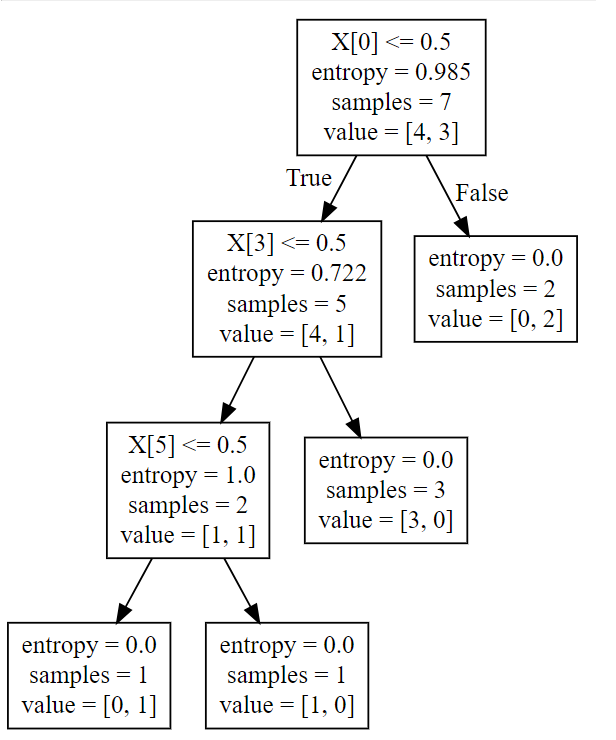
\includegraphics[width=0.3\linewidth,keepaspectratio]{mlcourse12}
\end{center}
\end{frame}

%%%%%%%%%%%%%%%%%%%%%%%%%%%%%%%%%%%%%%%%%%%%%%%%%%%%%%%%%%
\begin{frame}[fragile]\frametitle{Functions for calculating entropy and information gain}	
we have 9 blue balls and 11 yellow balls. Let ball have label 1 if it is blue, 0 otherwise.
\begin{lstlisting}
balls = [1 for i in range(9)] + [0 for i in range(11)]
\end{lstlisting}
Next split the balls into two groups:
\begin{lstlisting}
# two groups
balls_left  = [1 for i in range(8)] + [0 for i in range(5)] # 8 blue and 5 yellow
balls_right = [1 for i in range(1)] + [0 for i in range(6)] # 1 blue and 6 yellow
\end{lstlisting}
\end{frame}

%%%%%%%%%%%%%%%%%%%%%%%%%%%%%%%%%%%%%%%%%%%%%%%%%%%%%%%%%%
\begin{frame}[fragile]\frametitle{Question 5}	
\begin{center}
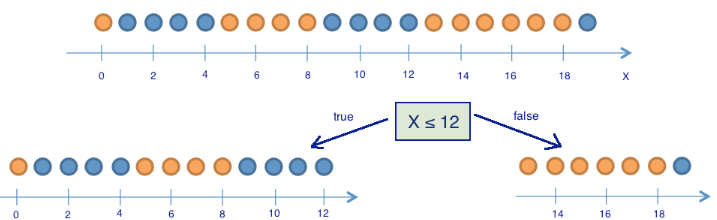
\includegraphics[width=0.8\linewidth,keepaspectratio]{mlcourse13}
\end{center}
Implement a function to calculate the Shannon Entropy
 \end{frame}

%%%%%%%%%%%%%%%%%%%%%%%%%%%%%%%%%%%%%%%%%%%%%%%%%%%%%%%%%%
\begin{frame}[fragile]\frametitle{Solution 5}	
\begin{lstlisting}
from math import log
    
def entropy(a_list):
    lst = list(a_list)
    size = len(lst) * 1.0
    entropy = 0
    set_elements = len(set(lst))
    if set_elements in [0,1]:
        return 0
    for i in set(lst):
        occ = lst.count(i)
        entropy -= occ/size * log (occ/size,2)
    return entropy
\end{lstlisting}

\end{frame}

%%%%%%%%%%%%%%%%%%%%%%%%%%%%%%%%%%%%%%%%%%%%%%%%%%%%%%%%%%
\begin{frame}[fragile]\frametitle{Tests}	

\begin{lstlisting}
print(entropy(balls)) # 9 blue and 11 yellow
print(entropy(balls_left)) # 8 blue and 5 yellow
print(entropy(balls_right)) # 1 blue and 6 yellow
print(entropy([1,2,3,4,5,6])) # entropy of a fair 6-sided die

>>
0.9927744539878084
0.961236604722876
0.5916727785823275
2.584962500721156
\end{lstlisting}

 \end{frame}
 
 %%%%%%%%%%%%%%%%%%%%%%%%%%%%%%%%%%%%%%%%%%%%%%%%%%%%%%%%%%
\begin{frame}[fragile]\frametitle{Tests}	
\begin{itemize}
\item What is the entropy of the state given by the list balls\_left? = 0.961
\item What is the entropy of a fair dice? (where we look at a dice as a system with 6 equally probable states)?  = 2.585
\end{itemize}

 \end{frame}

%%%%%%%%%%%%%%%%%%%%%%%%%%%%%%%%%%%%%%%%%%%%%%%%%%%%%%%%%%
\begin{frame}[fragile]\frametitle{Information Gain}	
\begin{lstlisting}
# information gain calculation
def information_gain(root, left, right):
    ''' root - initial data, left and right - two partitions of initial data'''
        
    return entropy(root) - 1.0 * len(left) / len(root) * entropy(left) \
                         - 1.0 * len(right) / len(root) * entropy(right) 
						 


\end{lstlisting}

\end{frame}

%%%%%%%%%%%%%%%%%%%%%%%%%%%%%%%%%%%%%%%%%%%%%%%%%%%%%%%%%%
\begin{frame}[fragile]\frametitle{Question 6}	
What is the information gain from splitting the initial dataset into balls\_left and balls\_right ?
\begin{lstlisting}
print(information_gain(balls, balls_left, balls_right))	
>>
0.16088518841412436
\end{lstlisting}

\end{frame}

%%%%%%%%%%%%%%%%%%%%%%%%%%%%%%%%%%%%%%%%%%%%%%%%%%%%%%%%%%
\begin{frame}[fragile]\frametitle{Best Feature to Split}	
\begin{lstlisting}
def best_feature_to_split(X, y):
    '''Outputs information gain when splitting on best feature'''
    out = []
    for i in X.columns:
        out.append(information_gain(y,y[X[i] == 0], y[X[i] == 1]))
    return out 
\end{lstlisting}

\end{frame}

%%%%%%%%%%%%%%%%%%%%%%%%%%%%%%%%%%%%%%%%%%%%%%%%%%%%%%%%%%
\begin{frame}[fragile]\frametitle{Test}	
\begin{lstlisting}
best_feature_to_split(df_train, y)

>>
[0.2916919971380598,
 0.005977711423774124,
 0.02024420715375619,
 0.46956521111470706,
 0.12808527889139454,
 0.005977711423774124,
 0.12808527889139454,
 0.46956521111470706]
\end{lstlisting}

\end{frame}

%%%%%%%%%%%%%%%%%%%%%%%%%%%%%%%%%%%%%%%%%%%%%%%%%%%%%%%%%%
\begin{frame}[fragile]\frametitle{Implement Decision Tree}	
\begin{lstlisting}
def btree(X,y):
    clf = best_feature_to_split(X, y)
    param = clf.index(max(clf))
    ly = y[X.iloc[:,param] == 0]
    ry = y[X.iloc[:,param] == 1]
    print ('Column_' + str(param) + ' N/Y?')
    print ('Entropy: ',entropy (ly), entropy (ry))
    print ('N count:',ly.count(),'/', 'Y count:',ry.count())
    if entropy (ly) != 0:
        left = X[X.iloc[:,param] == 0]
        btree(left, ly)
    if entropy (ry) != 0:
        right = X[X.iloc[:,param] == 1]
        btree(right, ry)
\end{lstlisting}

\end{frame}

%%%%%%%%%%%%%%%%%%%%%%%%%%%%%%%%%%%%%%%%%%%%%%%%%%%%%%%%%%
\begin{frame}[fragile]\frametitle{Test Decision Tree}	
\begin{lstlisting}
btree (df_train,y)

>>
Column_3 N/Y?
Entropy:  0.7219280948873623 0
N count: 5 / Y count: 2
Column_4 N/Y?
Entropy:  1.0 0
N count: 2 / Y count: 3
Column_0 N/Y?
Entropy:  0 0
N count: 1 / Y count: 1
\end{lstlisting}

\end{frame}